\chapter{Fundamentação Teórica}
\label{cap:fundamentacao-teorica}


\section{O terminal gráfico iX-T7F-2 (\acrshort{IHM})}
\label{sec:fundamentacao-equipamentos}

O terminal gráfico ou a\acrshort{IHM} da Altus, modelo iX-T7F-2, que aqui será abordada como equipamento de estudo, é chamada pela empresa de terminal de operação, e pode-se destacar algumas de suas características gerais, conforme Tabela \ref{tab:caracteristicasgerais}. 


\begin{table}[ht!]
	\Caption{\label{tab:caracteristicasgerais}Características gerais}
	\UECEtab{}{
		\begin{tabular}{ll}
			\toprule
			Característica & iX-T7F-2 \\
			\midrule \midrule
			Tamanho da tela & 7" (154,1mm x 85,9mm) \\
			Resolução da tela & 800x480 pixels (16:9) \\
			Visor & LCD-TFT 64K cores \\
			Tipo e vida útil do \textit{Backlight} & LED 20.000h \\
			\textit{Touchscreen} & Resistivo \\
			\midrule
			Memória de aplicação & 200MB \\
			Memória RAM & 128MB \\
			Relógio de tempo-real & sim \\
			\midrule
			Tensão de alimentação & 24V (18 a 32 $V_{DC}$) \\
			Fusível interno & 2A \\
			Máxima dissipação de potência & 9,6W \\
			\midrule
			Porta USB 2.0 (400mA) & 1 \\
			Porta Ethernet 10/100 Base-T & 1 \\
			COM1 & RS-232 (RTS/CTS) \\
			COM2 & RS-422/RS-485 \\
			COM3 & RS-232 \\
			COM4 & RS-485 \\
			\midrule
			Número de Tags & 800 \\
			Número de telas & 100 \\
			Alarmes & 400 \\
			Número de controladores de comunicação & 4 \\
			\bottomrule
		\end{tabular}
	}{
		\Fonte{Terminais de operação Série iX \cite{terminais_operacao_serie_ix}}
		\Nota{As portas COM1 e COM2 são alocadas em um mesmo conector, bem como a COM3 e a COM4. Assim, ao selecionar uma das portas de comunicação, a outra é desabilitada.}
	}
\end{table}




As dimensões e os conectores podem ser vistos na representação da Figura \ref{fig:ihm_dimensions}, em que deve-se notar que as portas COM1 e COM2 compartilham o mesmo conector DB9, da mesma forma que as portas COM3 e COM4 também compartilham um único conector DB9, desta forma, ao habilitar uma delas, a outra é desabilitada. 

\begin{figure}[ht!]
	\centering
	\Caption{\label{fig:ihm_dimensions} Dimensões e conectores}
	\UECEfig{}{
		\fbox{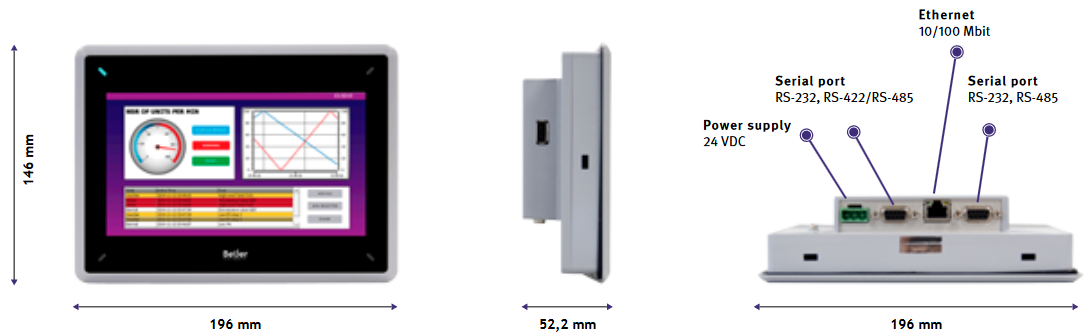
\includegraphics[width=14cm]{figuras/beijer-dimensions}}
	}{
		\Fonte{Beijer Eletronics}
	}
\end{figure}


Os terminais gráficos da Altus, são desenvolvidos e fabricados por uma empresa sueca, Beijer Electronics, Inc. que possui um foco em aplicações de comunicação, controle e interfaces homem-máquina para a industria. 
Por possuir uma abordagem transversal aos segmentos industriais, seus equipamentos destacam-se pela ampla gama de drives de comunicação disponíveis, incluindo não somente aqueles de domínio publico mas tambéms os proprietários. 
Aqui destacamos o Modbus definido pela MODICON, com os protocolos \textbf{Modbus Master RTU/ASCII} e \textbf{Modbus Slave RTU/TCP}.


A elaboração de projetos para o terminal gráfico é feita utilzando o software \textbf{iX Developer}, que pode ser obtido diretamente no site da Altus (www.altus.com.br), na aba \textbf{Suporte \& Downloads} >> \textbf{Downloads}, em \textbf{Central de Downloads} selecione somente a \textbf{Categoria: Softwares} e \textbf{Série: Série iX}. São listados os \textit{softwares}, Manuais e Apostilas disponíveis.


\subsection{Conexão para gravação de projeto no terminal gráfico/IHM}


De acordo com o documento \textbf{Terminais de Operação da Série iX} \cite{terminais_operacao_serie_ix}, o terminal gráfico pode receber um projeto para ser executado via \textit{pendrive} ou através da porta Ethernet, como ilustrado na Figura \ref{fig:pc_rot_ihm}, em que a conexão entre um computador e o terminal gráfico, possui um switch/roteador como intermediário da conexão. 
A conexão entre os dispositivos utiliza cabo de rede CAT5e e terminais seguindo o padrão EIA/TIA 568A. 


\begin{figure}[ht!]
	\centering
	\Caption{\label{fig:pc_rot_ihm}Conexão para \textit{download} da aplicação no terminal gráfico }
	\UECEfig{}{
		\fbox{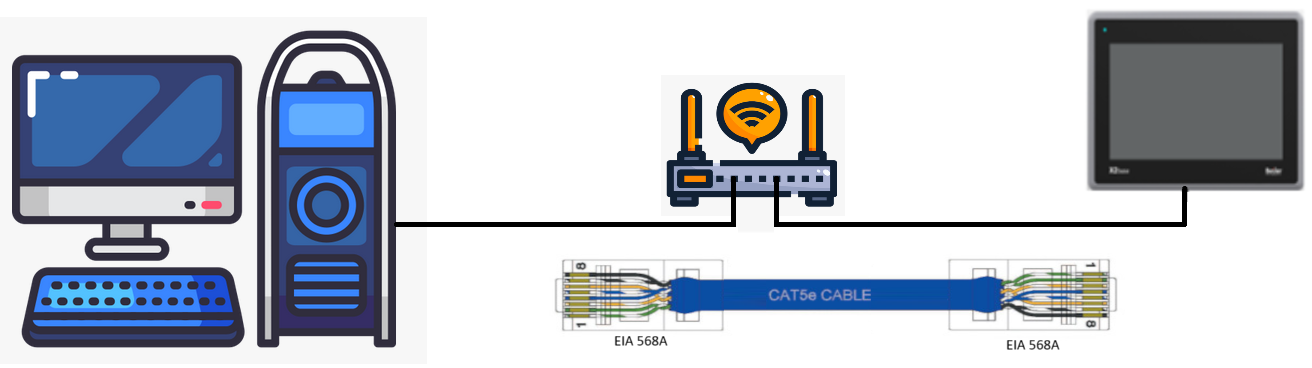
\includegraphics[width=14cm]{figuras/altus-pc_rot_ihm_cabo}}
	}{
		\Fonte{Próprio autor}
	}
\end{figure}


Da mesma forma, a Figura \ref{fig:pc_rot_ihm_wifi} ilustra a conexão feita por um notebook utilizando o \textit{Wi-Fi} como meio de comunicação. 

Note que, partindo do \textit{switch}/Roteador, cada ramo de comunicação utiliza um meio físico diferente, sendo que para o \textit{notebook} o meio é \textit{Wi-Fi} e para o terminal gráfico é cabo par-trançado direto.

O cabo par-trançado possui ambas as terminações no padrão EIA-568A, mas poderiam ser padrão EIA-568B, desde que em ambas as pontas.


\begin{figure}[ht!]
	\centering
	\Caption{\label{fig:pc_rot_ihm_wifi}Conexão via Wi-Fi para gravação de projeto no terminal gráfico}
	\UECEfig{}{
		\fbox{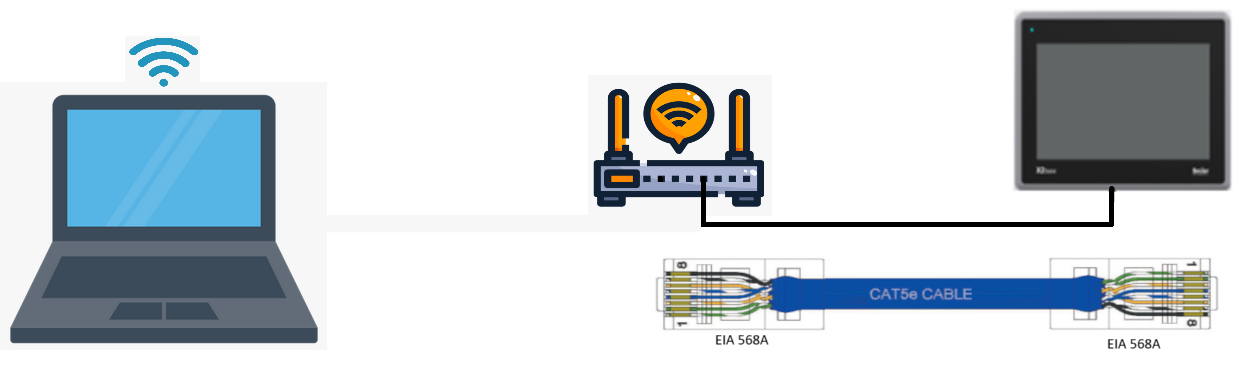
\includegraphics[width=14cm]{figuras/altus-pc_rot_ihm_wifi}}
	}{
		\Fonte{Próprio autor}
	}
\end{figure}


Pode-se ainda fazer a conexão direta entre o computador/notebook e o terminal gráfico utilizando um cabo de rede padrão crossover.

No caso do cabo de rede de par-trançado padrão crossover, uma das terminações é montada com o padrão EIA-568A enquanto a outra terminação é montada no padrão EIA-568B.



\begin{figure}[ht!]
	\centering
	\Caption{\label{fig:pc_ihm_cabocross}Conexão direta para \textit{download} de projeto no terminal gráfico}
	\UECEfig{}{
		\fbox{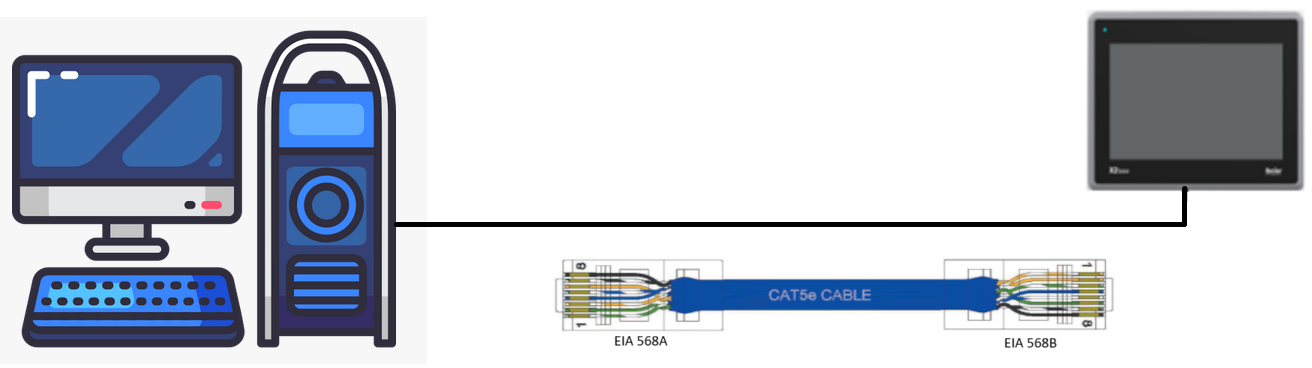
\includegraphics[width=14cm]{figuras/altus-pc_ihm_cabocross}}
	}{
		\Fonte{Base de conhecimento - Altus \cite{ixdev_download}}
	}
\end{figure}


Mais informações podem ser obtidas na Plataforma Base de conhecimento da Altus \cite{ixdev_download}, inclusive para a realização de \textit{upload} de programa contido no terminal gráfico de volta ao iX Developer.  






\section{Conexão entre o terminal Gráfico/IHM e o CLP}

A operação do terminal gráfico, execução do projeto nele gravado, ocorre mediante a sua comunicação com um controlador, normalmente um \acrshort{CLP}, mas pode ser qualquer dispositivo que implemente um dos protocolos disponíveis. 

O protocolo de comunicação que será aqui utilizado é o Modbus e o controlador é o \acrshort{CLP} da linha DUO da Altus, montado em um kit didático, o \acrshort{TB}131 (\acrlong{TB}). 

Como exemplo diferente ao \acrshort{CLP}, poderíamos utilizar uma placa de desenvolvimento contendo um microcontrolador, como um Arduino, devidamente programado e com o protocolo Modbus implementado. Esta é uma outra possibilidade com real viabilidade. 

O protocolo Modbus foi desenvolvido pela Modicom nos primórdios da automação, no final da década de 70. 
Por ser um protocolo aberto, pode ser livremente implementado pelos diversos fabricantes de equipamentos, mesmo que praticamente todos os desenvolvedores possuam o seu próprio protocolo. 
Desta forma o Modbus se tornou uma "língua franca", falada por praticamente todos os equipamentos do mercado, possibilitando assim, que em uma rede possam interagir equipamentos dos mais diversos fabricantes. 

Mais informações de forma didática sobre detalhes do protocolo Modbus podem ser encontradas no site Automação e Cartoons \cite{automacao_cartoon} ou ainda diretamente da insituição que gerencia o padrão atualmente, Modbus.org \cite{modbus_org}.




A comunicação entre a \acrshort{IHM} e o \acrshort{TB}131 pode ser realizada como ilustrado na Figura \ref{fig:connect_ihm_clp},
%
%e \ref{fig:connect_ihm_clp_cabosimples}. O meio físico aqui utilizado é RS-485, por ser de uso mais difundido em aplicações industriais.
%
conforme recomendação nos manuais da Altus \cite{connect_ihm_tb131}. 
Nela, um módulo de interface, PO8525 \cite{po8525} é utilizado entre o terminal gráfico e o controlador. 





\begin{figure}[ht!]
	\centering
	\Caption{\label{fig:connect_ihm_clp}Conexão entre IHM e CLP}
	\UECEfig{}{
		\fbox{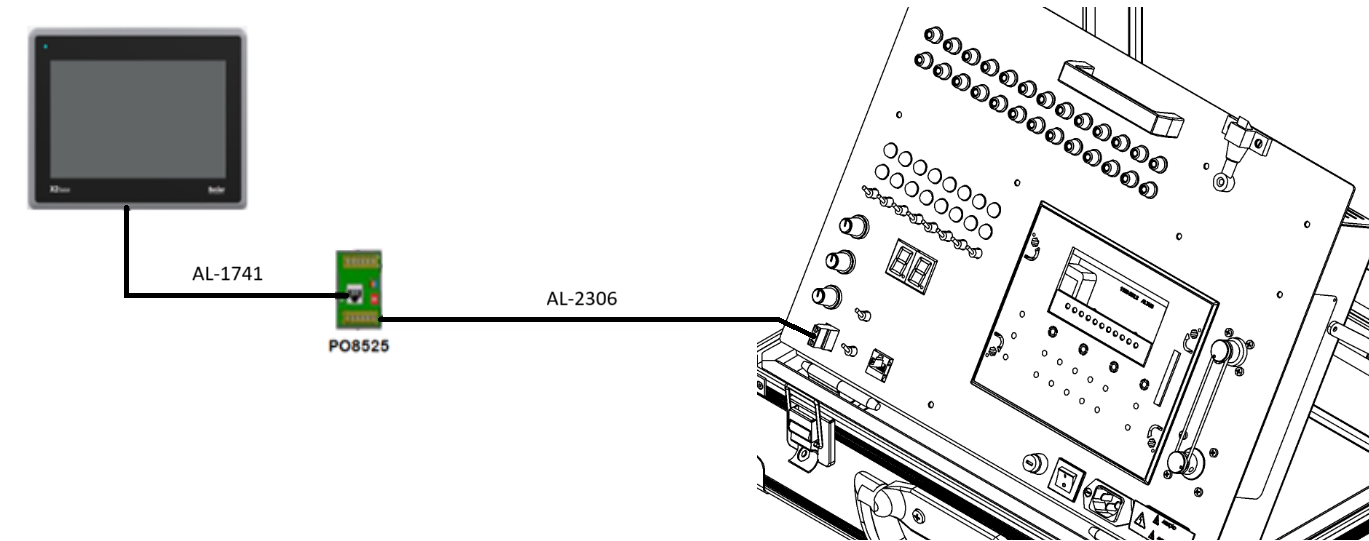
\includegraphics[width=14cm]{figuras/altus-conexao-ix_t7f_2-tb131}}
	}{
		\Fonte{Adaptado de \cite{connect_ihm_tb131}}
	}
\end{figure}


Entre o terminal gráfico e o módulo de interface, basicamente, pode-se utilizar um cabo com terminal DB9 em uma extremidade e RJ45 na outra \cite{al1741} e entre o módulo de interface e o TB131 um cabo no padrão AL-2306 \cite{al2306}.




Já entre o módulo de interface e o TB131 temos um par de cabos simples, trançado, blindado ou não, para fazer o meio físico RS-485, conforme Figura \ref{fig:connect_ihm_clp_cabosimples}. 
Desta forma, pode-se adaptar uma conexão ponto-a-ponto para estudo, utilizando um conector DB9 Macho para o terminal conectado à \acrshort{IHM} na COM2 ou COM4 (RS-485), conforme Tabela \ref{tab:caracteristicasgerais}, e para um ligação direta nos bornes do TB131, um simples decape nas pontas do fio.


\begin{figure}[ht!]
	\centering
	\Caption{\label{fig:connect_ihm_clp_cabosimples}Conexão direta entre IHM e CLP}
	\UECEfig{}{
		\fbox{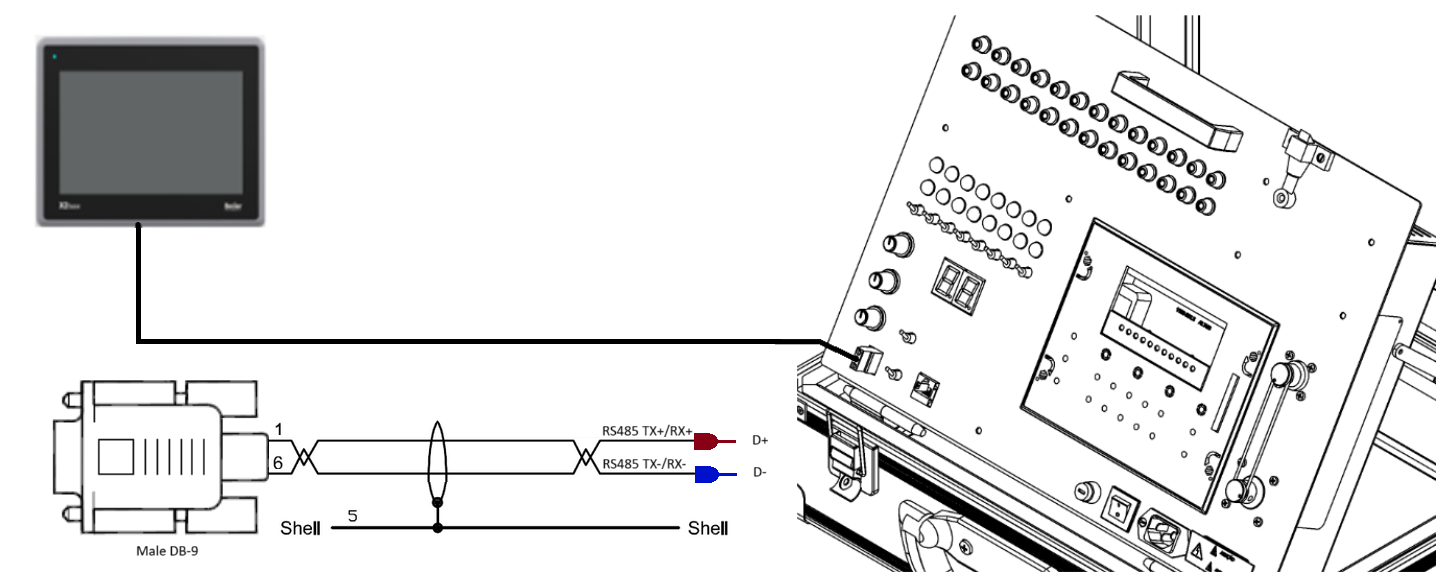
\includegraphics[width=14cm]{figuras/altus-conexao-ihm-tb131-cabosimples}}
	}{
		\Fonte{Adaptado de \cite{connect_ihm_tb131}}
	}
\end{figure}

O ponto que requer atenção é a polaridade do cabo, pois o terminal 1 do DB9 é o Sinal (+) da comuniação, enquanto o terminal 6 do DB9 é o Sinal (-), respectivamente, conectados em D+ e D- no TB131. 

Caso seja utilizado um par de cabos com malha, esta deve ser conectada ao Referencial no pino 5 do conector DB9 e no GND do conector RS-485 do TB131. 









\section{Kit didático CLP DUO - \acrlong{TB} 131 (\acrshort{TB}131)}


O kit didático possui uma interface de comunicação RS-485 que pode ser acessada habilitando a porta de comunicação serial COM2, conforme Figura \ref{fig:config_com}, através do \textit{software} de programação \textbf{Master Tool IEC}. 

A configuração da comunicação serial pode ser acessada na \textbf{Aba Recursos} >> \textbf{Configurações do CP} >> \textbf{Comunicação[FIX]} >> \textbf{COM 2[FIX]} >> Clique com o botão direito do mouse >> \textbf{Substituir elemento}.
Podem ser escolhidas as opções MODBUS Mestre, \textbf{MODBUS Escravo} ou Protocolo Genérico \cite{tb131}. 


\begin{figure}[ht!]
	\centering
	\Caption{\label{fig:config_com}Configuração de porta de comunicação Modbus}
	\UECEfig{}{
		\fbox{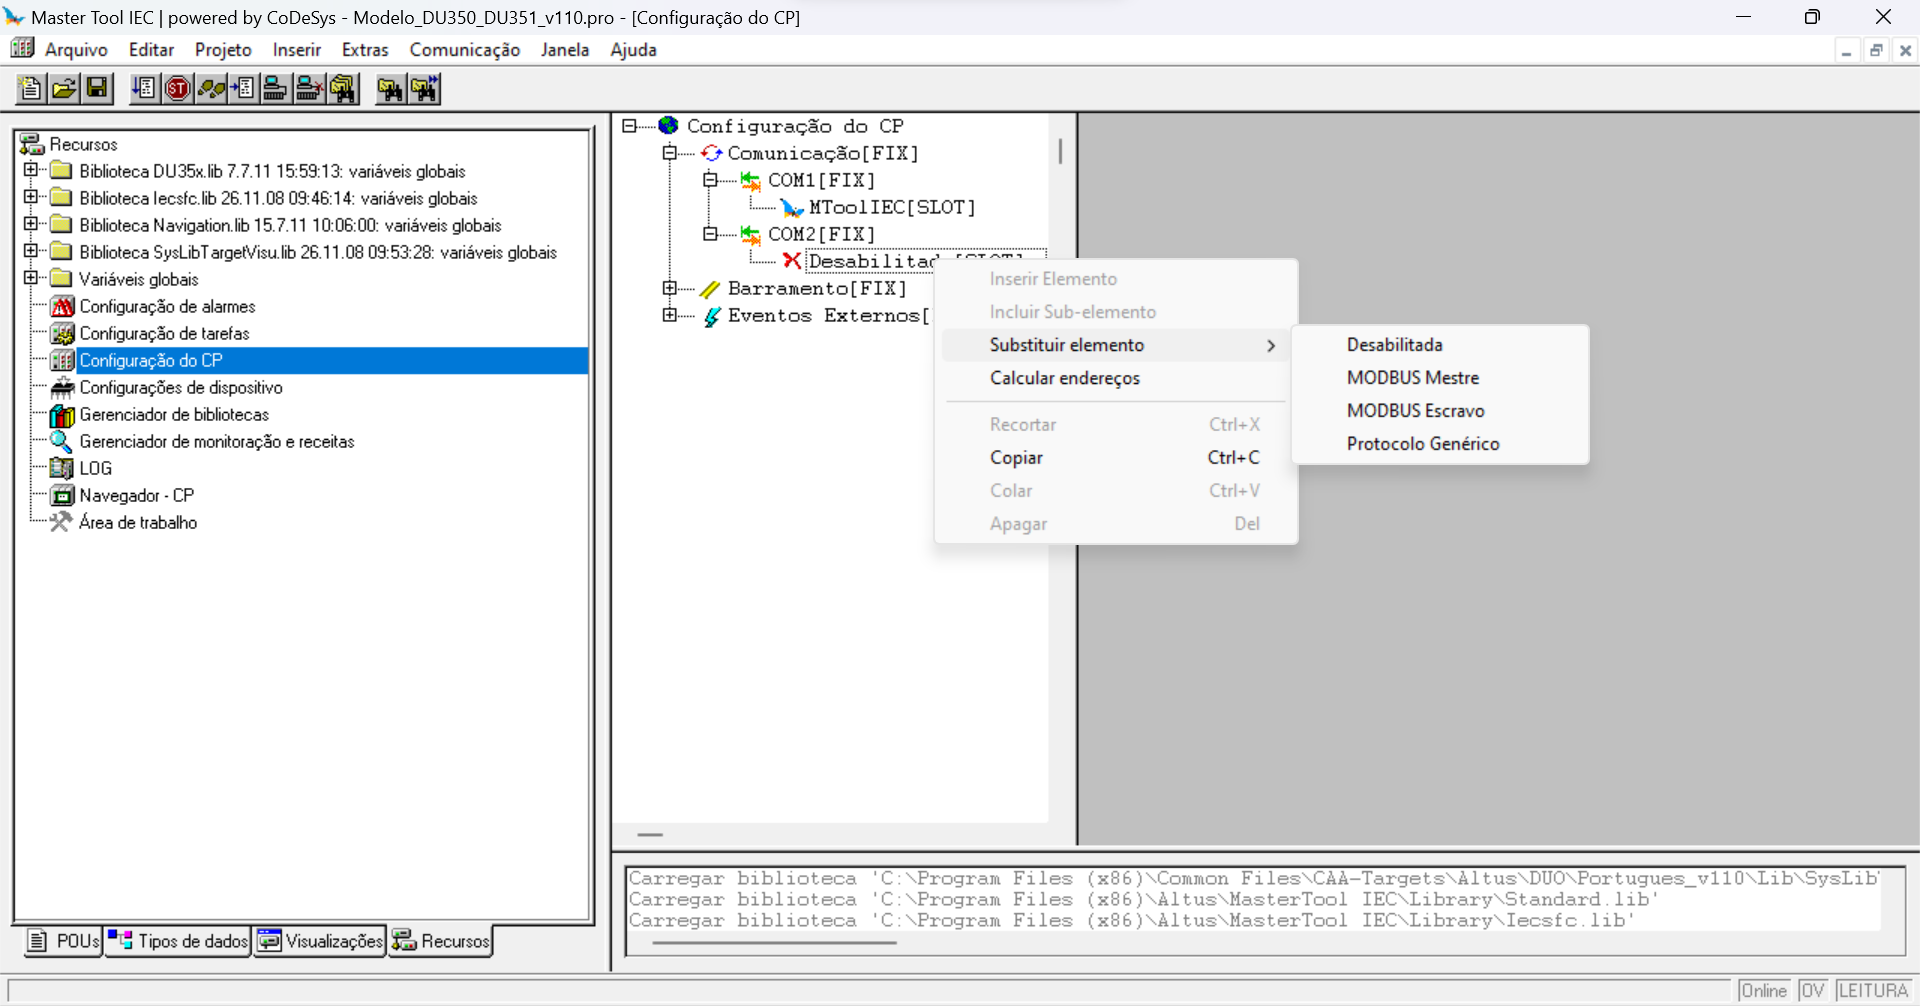
\includegraphics[width=14cm]{figuras/tb131-recursos-config-com}}
	}{
		\Fonte{Próprio autor}
	}
\end{figure}


Ao configurar a porta de comunicação como \textbf{MODBUS Escravo}, pode-se parametrizar o seu endereço como na Figura \ref{fig:com_modbus_slave_address}.

\begin{figure}[ht!]
	\centering
	\Caption{\label{fig:com_modbus_slave_address}Endereçamento de Registradores e Funções Modbus}
	\UECEfig{}{
		\fbox{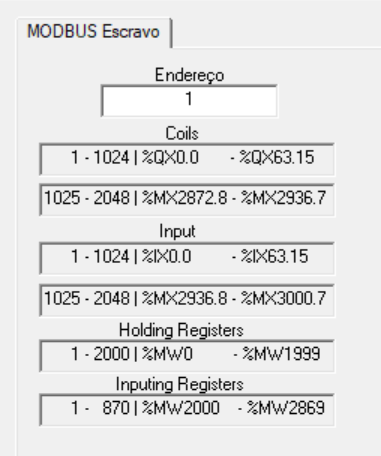
\includegraphics[width=6cm]{figuras/tb131-modbus_slave_address}}
	}{
		\Fonte{Próprio autor}
	}
\end{figure}


O endereçamento do escravo Modbus pode ser parametrizado com valor dentro do intervalo de 1 a 247, conforme o Manual de utilização da Série DUO \cite{manual_tb131}.


Para o acesso às entradas e saídas digitais endereçadas em \%IX0.0 até \%IX0.7 e \%QX1.0 até \%QX1.7, mapeadas nas chaves e LEDs no painel do TB131, não é necessária qualquer outra configuração além de habilitar a comunicação MODBUS na COM2, pois as funções Modbus acessam diretamente os endereços correspondente às entradas e saídas digitais. 

O termo Mestre-Escravo, historicamente utilizado pra denominar os elementos que se comunicam em uma rede, 
está sendo substituido pelo termo Cliente-Servidor, 
alinhando-se com as boas práticas de eliminação de linguagem inapropriada  \cite{client_server}.




%\cite{tb131}





% Manual de utilização iX-Developer \cite{ix_manual}


% \subsection{Características técnicas}

%\section{Protocolo de comunicação}
%\label{sec:fundamentacao-protocolo_comunicacao}

%\subsection{Características do sinal}

%\subsection{Configuração de comunicação Modbus}

%Os terminais de operação podem ser acessados em \cite{terminais_operacao_serie_ix}.

%Para os cabos de comunicação acesso o \cite{al1741} e \cite{al2306} bem como o derivador pode ser acessado em \cite{po8525}


% TrainingBoxDuo \cite{tb131}.
